\begin{document}
\title{Übungsblatt~3}
\subtitle{Sätze}
\maketitle

\section*{Lernziele}
\begin{itemize}
	\item Ziele des Schlüsselzugriffs
	\item Hashing als Methode des Schlüsselzugriffs
	\item Wahl der Hashfunktion und Überlaufbehandlung beim Hashing
	\item Lineares Hashing
\end{itemize}


\begin{normalText}
\section*{Literatur}
\HaerderNintyNine{7.4, 7.5, 7.6}

\ElmasriSeventh{16.8}
\end{normalText}

\section{Fragen zur Vorlesung}
\begin{enumerate}[a)]
	\item Wozu dient der Datenbankpuffer?

	\begin{solution}
	Der Datenbankpuffer dient dem Zwischenspeichern von Daten im Hauptspeicher. Ziel ist es, die Performance zu erhöhen, indem man Blöcke nicht erst von der langsamen Platte lesen muss, sondern sie im schnellen Hauptspeicher vorhält.
	\end{solution}


	\item Warum verwendet man nicht einfach die Pufferverwaltung des Betriebssystems?

	\begin{solution}
	\begin{itemize}
		\item Tut man ja. Die Pufferverwaltung des BS ist weiterhin aktiv und kann Daten auf die Platte auslagern, von denen das DBMS glaubt, sie seien im Speicher.

		\item Das Betriebssystem weiß weniger über die anwendungsspezifischen Zugriffsmuster und kann daher keine optimale Strategie anwenden. Für unseren speziellen Anwendungsfall können wir es besser. Das ist der Hauptgrund, warum man sich nicht alleine auf das BS verlässt. Außerdem bietet das Betriebsystem nicht die Schnittstellen, die für die anderen Schichten gebraucht werden (z.\,B. Transaktionssystem).

		\begin{note}
		\item Weitere Überlegung (technisch, müssen die Teilnehmer nicht wissen): Die Pufferverwaltung des BS stellt jedem Programm einen (virtuellen) Adressraum zur Verfügung, den dieses nutzen kann. Es kann dann Seiten dieses virtuellen Adressraumes an beliebige Stellen des physischen Adressraumes schieben oder sie gar auf die Platte auslagern. Die Anwendung sieht davon nichts, sie greift einfach auf Adressen im virtuellen Adressraum zu. In unserem Fall hieße das, wir würden die gesamte Datenbank in den virtuellen Adressraum kopieren und das BS entscheiden lassen, welche Frames/Seiten davon wirklich im Hauptspeicher liegen. Dank \texttt{mmap()} o.\,ä. geht das sogar schnell. Allerdings ist bei 32-bit-Architekturen der Adressraum auf 4\,GiB beschränkt, das ist viel zu wenig. Unter 64-bit Linux stehen pro
Prozess 128\,TiB virtueller Adressraum zur Verfügung, unter 64-bit Windows 8\,TiB. Auch das kann von großen Datenbanken überschritten werden. Man muss also entscheiden, welche Frames im virtuellen Adressraum liegen sollen. Und das ist bereits wieder eine eigene Pufferverwaltung.
		\end{note}
	\end{itemize}
	\end{solution}


	\item Welche Probleme kann ein Puffer im Fehlerfall (z.\,B. Stromausfall) verursachen? Wie kann man damit umgehen?

	\begin{solution}
	Wenn nicht gespeicherte Änderungen im Puffer liegen, gehen sie verloren. Das ist nicht zu ändern und immer unangenehm, besonders aber wenn Inkonsistenzen auftreten.

	Beispiele:
	\begin{itemize}
		\item Änderungen in verzweigten Strukturen (Listen Element verschieben, B-Baum-Splitt): Nachfolger sind schon persistiert, Vorgänger noch nicht $\rightarrow$ es fehlt die Verzweigung, der Nachfolger kann nicht gefunden werden.
		\item Freispeicherverwaltung (vgl. Übung 4 -- Sätze): Ein Satz wurde in einen Block eingefügt, die Freispeichertabelle ist noch nicht angepasst.
		\item Wir überweisen Geld. Abbuchung ist schon auf der Platte, Gutschrift noch nicht $\rightarrow$ Geldvernichtung
	\end{itemize}
	Minimalziel ist es daher immer, einen konsistenten Zustand zu gewährleisten. Ab da können die Anwendungen ihre Arbeit ggf. noch mal machen. Das schafft man z.B. indem man alte Blöcke nicht überschreibt, sondern den neuen Inhalt in neue Blöcke schreibt und atomar umschaltet.

	Bei den ersten beiden Beispielen, weiß das DBMS, welche Änderungen zusammengehören und wieder zu einem konsistenten Zustand führen. Im dritten Beispiel weiß das nur die Anwendung $\rightarrow$ Transaktionen, siehe später
	\end{solution}


	\item Was ist der Unterschied zwischen direkter und indirekter Seitenzuordnung? Was ist der Unterschied zwischen direkter und indirekter Seiteneinbringung?

	\begin{solution}

	\paragraph{Block, Seite und Kachel}
	Zunächst unterscheiden wir die Begriffe Block, Seite und Kachel:
	\begin{description}
		\item[Block] Block auf der physischen Festplatte, es werden immer ganze Blöcke gelesen und geschrieben und von der Platte in den Hauptspeicher transportiert und umgekehrt.
		\item[Kachel] Eine Kachel ist der Platz für einen Block im Datenbankpuffer. %% im (virtuellen) Hauptspeicher
		\item[Seite] Eine Seite ist die Adressierungseinheit an der Pufferschnittstelle. Eine Seite wird auf Blöcke abgebildet und ist genauso groß wie ein Block. Die höhere Softwareschicht arbeitet nur noch mit Seiten.
	\end{description}


	\paragraph{Seitenzuordnung}
	\begin{description}
		\item[Direkte Seitenzuordnung] bedeutet, dass aufeinanderfolgende Seiten auch in aufeinanderfolgenden Blöcken einer Datei abgelegt werden. Man muss sich also nur die erste Blocknummer für ein Segment merken und kann die Blocknummern für alle Seiten des Segments ausrechnen.

		Das hat nichts mit den Kacheln im Puffer zu tun. Im Puffer können die Seiten deshalb trotzdem komplett verstreut liegen und auch einzeln verdrängt werden. Der Puffer merkt sich zu jeder Kachel, welche Seite darin liegt und kann durch die Seitenzuordnung ermitteln, in welchen Block sie geschrieben werden muss.

		\item[Indirekte Seitenzuordnung] heißt, dass über eine Tabelle festgelegt wird, welche Seite auf welchen Block einer Datei abgebildet wird. Hintereinanderliegende Seiten müssen also nicht mehr in aufeinanderfolgenden Blöcken liegen.
	\end{description}

	Direkt ist schneller und benötigt weniger Verwaltungsdaten, dafür ist es aber auch unflexibler.

	\paragraph{Einbringstrategie}
	Die grundlegende Idee ist, dass speichern auf der Festplatte beim Verdrängen aus dem Puffer nicht notwendigerweise sofort ein Einbringen in den Datenbestand sein muss.

	\begin{description}
		\item[Direkte Seiteneinbringung] heißt, dass Seiten, die auf die Platte gespeichert werden, weil sie aus dem Puffer verdrängt werden, sofort in den Datenbestand eingebracht werden. Das heißt, alle Zeiger und Zuordnungstabellen zeigen sofort auf die neuen Daten. Das geschieht im allgemeinen einfach dadurch, dass die Seite wieder in den Block geschrieben wird, aus dem sie gelesen wurde.
		\item[Indirekte Seiteneinbringung] heißt, geänderte Seiten werden nicht sofort, wenn sie aufgrund der Verdrängung aus dem Puffer auf die Platte gespeichert werden, in den Datenbestand eingebracht. Dies geschieht erst später, z.B. nach einer Datenänderung erst dann, wenn alle Daten der Transaktion geändert sind und auch die Seiten der zugehörigen Indexstrukturen (z.B. B-Bäume) angepasst sind. Hierzu werden die verdrängten Seiten zunächst in neue Blöcke geschrieben und diese erst später durch Änderung von Verwaltungsstrukturen als zum Datenbestand gehörig gekennzeichnet.
	\end{description}

Indirekte Seiteneinbringung ist aufwändiger, bietet aber den Vorteil, dass man den alten Block im Fehlerfall wiederherstellen kann, da er ja noch existiert.
 Direkte Seiteneinbringung hingegen ist von sich aus nicht fehlertolerant. Fehlertoleranz kann z.\,B. über das Führen eines Logs erreicht werden. Die Wiederherstellung muss im Fehlerfall dann das Log auswerten und Änderungen rückgängig machen.

Die Kombination indirekter Seiteneinbringung mit direkter Seitenzuordnung wird beispielsweise durch das Twin-Slot-Verfahren (siehe VL-Folie~\TwinSlot) realisiert.
\end{solution}
\end{enumerate}


\beamertxt{\pagebreak}
\section{Blockung von Sätzen}
\begin{enumerate}[a)]
	\item Entwickeln Sie jeweils eine Formel, mit welcher sich
	\begin{enumerate}[i)]
		\item der Blockungsfaktor $\mathit{bfr}$ eines Blocks (Ganzzahl, die angibt, wieviele Sätze pro Block gespeichert werden können), sowie
		\item der ungenutzte Speicherplatz am Ende eines Blocks
	\end{enumerate}
	berechnen lässt. Gehen Sie dabei davon aus, dass Ihre Sätze eine feste Länge $R$ haben, die kleiner oder gleich der Blockgröße $B$ ist und dass die Sätze nicht blockübergreifend abgespeichert werden.

	\begin{solution}
	\begin{enumerate}[i)]
		\item Blockungsfaktor: $\mathit{bfr} = \lfloor\frac{B}{R}\rfloor$
		\item Ungenutzter Speicherplatz: $B - (\mathit{bfr} \cdot R)$
	\end{enumerate}
	\end{solution}


	\item Geben Sie den Blockungsfaktor sowie den ungenutzten Speicherplatz an, bei einer Blockgröße von 4~KiB \nt{(1 Kibibyte = 1024 Byte)} und einer festen Satzlänge von
	\begin{enumerate}[i)]
		\item 67~Byte
		\item 109~Byte
		\item 237~Byte \selbst
	\end{enumerate}
	Gehen Sie auch hier wieder von keinen blockübergreifenden Sätzen aus.

	\begin{solution}
	\begin{enumerate}[i)]
		\item Blockungsfaktor: 61, ungenutzter Speicherplatz: 9~Byte
		\item Blockungsfaktor: 37, ungenutzter Speicherplatz: 63~Byte
		\begin{note}
			\item Blockungsfaktor: 17, ungenutzter Speicherplatz: 67~Byte
			\end{note}
	\end{enumerate}
	\end{solution}


	\item Gegeben sind die folgenden Satzlängen in Byte:

	397, 134, 80, 243, 175, 298, 153, 414, 38, 259, 49

	Wie viele Blöcke der Größe 512~Byte benötigen Sie, um diese Sätze in der angegebenen Reihenfolge abzuspeichern? Berechnen Sie außerdem den durchschnittlich ungenutzten Speicherplatz pro Block in Byte.

	\begin{solution}
	\begin{tabular}{ | p{2.4cm} | p{1.1cm} | p{1.1cm} | p{1.1cm} | p{1.1cm} | p{1.1cm} | p{1.1cm} | p{1.3cm} | }
		\hline
		Blocknummer 						&	1 			& 		2 						& 		3					&		4 			& 		5 					& 		6 				& 	Summe	\\
		\hline
		Sätze 									&	397		&		134, 80, 243 	&		175, 298		&		153		&		414, 38		&		259, 49	&				\\
		\hline
		genutzter Speicherplatz 		& 	397 		& 		457 					& 		473 				& 		153 		&		452 				& 		308			& 	2240 	\\
		\hline
		ungenutzter Speicherplatz 	& 	115 		& 		55 					& 		39 				& 		359 		& 		60 				& 		204 			& 	832 		\\
		\hline
	\end{tabular}

	Um den durchschnittlich ungenutzten Speicherplatz pro Block zu berechnen, summiert man den ungenutzten Speicherplatz der einzelnen Blöcke auf und teilt diesen anschließend durch die Anzahl der Blöcke. Im obigen Beispiel ergibt sich:\\ $\frac{115+55+39+359+60+204}{6} = \frac{832}{6} \approx 138,67$ (ca. 27,1\,\%)


	\paragraph{Zusatzfrage optimale Verteilung}
	Wie sähe eine optimale Verteilung aus?

	Wir können höchstens einen Block einsparen (da insgesamt weniger als 1024~Byte leer sind). Der letzte Block sollte möglichst den ganzen Freispeicher enthalten (oder auch irgendein anderer Block).

	Einfacher Algorithmus: wir fügen immer in den ersten Block ein, in dem noch genug Platz ist. Das ergibt:

	\begin{tabular}{ | p{2.4cm} | p{1.1cm} | p{1.1cm} | p{1.1cm} | p{1.1cm} | p{1.1cm} | p{1.3cm} | }
		\hline
		Blocknummer						& 		1 				& 		2 							& 		3 					& 		4 					& 		5 			& 	Summe		\\
		\hline
		Sätze 									& 		397, 80 	& 		134, 243, 38, 49 	& 		175, 298 		&		153, 259		&		414  	& 					\\
		\hline
		genutzter Speicherplatz 		& 		477 			& 		464 						& 		473 				& 		412 				& 		414 		& 	2240 		\\
		\hline
		ungenutzter Speicherplatz 	& 		35 			& 		48 						& 		39 				& 		100 				& 		98 		& 	320			\\
		\hline
	\end{tabular}

	Daduch ergibt sich für den durchschnittlich ungenutzten Speicherplatz pro Block: $\frac{35+48+39+110+98}{5} = \frac{320}{5} = 64$  (12,5\,\%)

	Damit ist der Block schon eingespart. Man muss jetzt aber schnell den ersten freien Block finden können. Der Platz ist nicht optimal zusammenhängend, aber das ist schwierig. Optimale Lösung benötigt Kenntnis über alle Sätze und ist zu aufwändig zu berechnen. Stattdessen können nur verschiedene Heuristiken verwendet werden (first match, last match, best match etc.).

	\paragraph{Zusatzfrage Blockgrößen}
	Letzte Woche haben wir Blockgrößen in Dateisystemen diskutiert. Im Mittel wird dort je Datei ein halber Block verschwendet. (Jede Dateigröße ist gleich wahrscheinlich, also besteht auch die gleiche Wahrscheinlichkeit 0, 1/n-1, 2/n-1, \ldots n-2/n-1 Platz im letzten Block zu verschwenden.)

	$\Rightarrow$ Kleine Blöcke verschwenden weniger Platz.

	Wie ist das nun mit den Satzdateien? Nehmen wir erstmal Sätze fester Länge an. %Im Mittel verschwenden wir einen halben Satz pro Block (analoge Begründung zu eben).
	Wir verschwenden immer weniger als einen Satz pro Block. Wäre noch Platz f\"ur einen weiteren Satz, w\"urde dieser Platz f\"ur den n\"achten Satz benutzt werden.
	Bei großen Blöcken ist die Wahrscheinlichkeit, dass ein Satz noch in den Block passt größer.

	$\Rightarrow$ Große Blöcke verschwenden weniger Platz.

	Wie passt das zusammen?
	\begin{itemize}
		\item Auch bei der Satzdatei ist im Mittel der letzte halbe Block leer. Hier ändert sich also nichts
		\item Eine normale Datei kann man als sequenzielle Satzdatei mit Sätzen der Länge 1 auffassen,
				hier kann weniger als ein Satz nicht verschwendet werden, da nur ganze Bytes verschwendet werden k\"onnen
				(weil es kein Satzkonzept gibt; die Daten werden einfach hintereinander geschrieben). Das ist gerade der Unterschied.
		\item Da Dateisysteme viele kleine Dateien beeinhalten (z.\,B. Konfigurations- oder kleine Textdateien), ist das erste Problem hier größer. Das zweite ist nicht existent. Also haben kleine Blöcke Vorteile
		\item Bei Datenbanken haben wir relativ wenige Dateien, aber viele Blöcke. (Alle Sätze gleichen Typs liegen i.\,A. in nur einer Datei. Ausnahme: Einteilung von Oracle: table spaces in data files.) Dadurch ist das erste Problem kleiner, das zweite überwiegt. Also haben hier eher große Blöcke Vorteile.
	\end{itemize}
	\end{solution}
\end{enumerate}





\section{Wechselpuffertechnik}
Betrachten Sie die Wechselpuffertechnik, die im Skript auf den Folien~\Wechselpuffertechnik~beschrieben ist. In welchem Verhältnis muss die Zeit, die für die Bearbeitung eines Blocks im Hauptspeicher benötigt wird, zur Zeit stehen, die für den Transfer dieses Blocks in den Hauptspeicher benötigt wird, damit die CPU voll ausgelastet ist? Gehen Sie hierbei auch auf die Ergebnisse aus Aufgabe~2 des zweiten Übungsblattes ein.

Gehen Sie davon aus, dass es nur eine CPU gibt, dass diese nur für die Blockbearbeitung und nicht für den Blocktransfer beansprucht wird und dass die Blöcke vom Externspeicher nur gelesen werden müssen.

\begin{solution}
Die Bearbeitungszeit für einen Block im Hauptspeicher muss mindestens so groß sein wie die Zeit, die für den Transfer eines Blocks vom Externspeicher in den Hauptspeicher benötigt wird.
Dann ist der für die CPU nächste zu bearbeitende Satz bereits vorhanden, sobald diese mit dem vorherigen fertig ist.

Im Allgemeinen Fall mit Transferdauer pro Block $a$ und Bearbeitungszeit pro Block $b$ gilt damit:
\begin{itemize}
	\item ohne Wechselpuffer $n(a+b)$
	\item mit Wechselpuffer $n \cdot \max(a, b)+\hspace{-20pt}\underbrace{\min(a, b)}_{f"ur~den~n-ten~Block}\hspace{-20pt} = a + b + (n-1) \cdot \max(a,b)$
\end{itemize}

Referenz auf das zweite Übungsblatt:
Wenn die Blöcke verstreut auf der Platte liegen, ist es nahezu unmöglich, die CPU auszulasten. Denn welche Operation ist so langsam, dass sie über 5\,ms (= mittlere Zugriffszeit (Seek- und Rotationslatenz-Zeit), die dann für jeden Block anfällt) CPU-Zeit braucht?

Somit gilt: Sind wir I/O-bound und ist die Transferdauer pro Block $a$, sowie die Bearbeitungszeit pro Block $b$, so braucht man für $n$ Blöcke
\begin{itemize}
	\item ohne Wechselpuffer $n(a+b)$
	\item mit Wechselpuffer $n \cdot a+\hspace{-35pt}\underbrace{b}_{f"ur~den~n-ten~Block}$
\end{itemize}

Je kleiner also das Verhältnis $\frac{b}{a}$, desto geringer fällt der Zugewinn bei der CPU-Auslastung aus. Die Praxis ist natürlich komplizierter; die Dauern gelten ja nur im Mittel.





\end{solution}



\beamertxt{\pagebreak}
\section{TID angewandt 1}
\label{sec:TID_angewandt1}
Betrachten Sie die unten skizzierte Ausgangssituation: Es sind Blöcke mit einer Größe von 48~Byte (ein Byte ist hier jeweils durch ein Kästchen repräsentiert) gegeben. Block~0 enthält zum Ausgangszeitpunkt genau 2 Sätze: TID(0, 0) mit der Länge 7 und TID(0, 1) mit der Länge 17.

Gehen Sie von einem stark vereinfachten TID-Konzept aus: Legen Sie lediglich die Nutzdaten der Sätze selbst, bei einem Überlauf die neue TID eines Satzes und die Indexeinträge für die Sätze in den Blöcken ab. Zusätzliche Informationen, wie den normalerweise üblichen TID-Header und Längeninformationen zu jedem Satz, können Sie vernachlässigen. Nehmen Sie an, dass für einen Indexeintrag genau 1~Byte, und für eine TID genau 2~Byte Speicherplatz benötigt werden. Darüber hinaus müssen Sie sich auch keine Gedanken darüber machen, wie erkannt wird, ob es sich bei den abgelegten Daten um Nutzdaten, eine TID oder einen Indexeintrag handelt.

\begin{beamerText}
\pagebreak

\begin{itemize}
\setlength{\itemindent}{17.6pt}
	\item Größe eines Indexeintrags 1~Byte
	\item Größe einer TID 2~Byte
	\end{itemize}
\end{beamerText}
\begin{enumerate}[a)]

	\item Fügen Sie in die Skizze Sätze mit folgenden Längen nacheinander ein und geben Sie jeweils die zugehörige TID an: 12, 10, 18.

	\begin{center}
	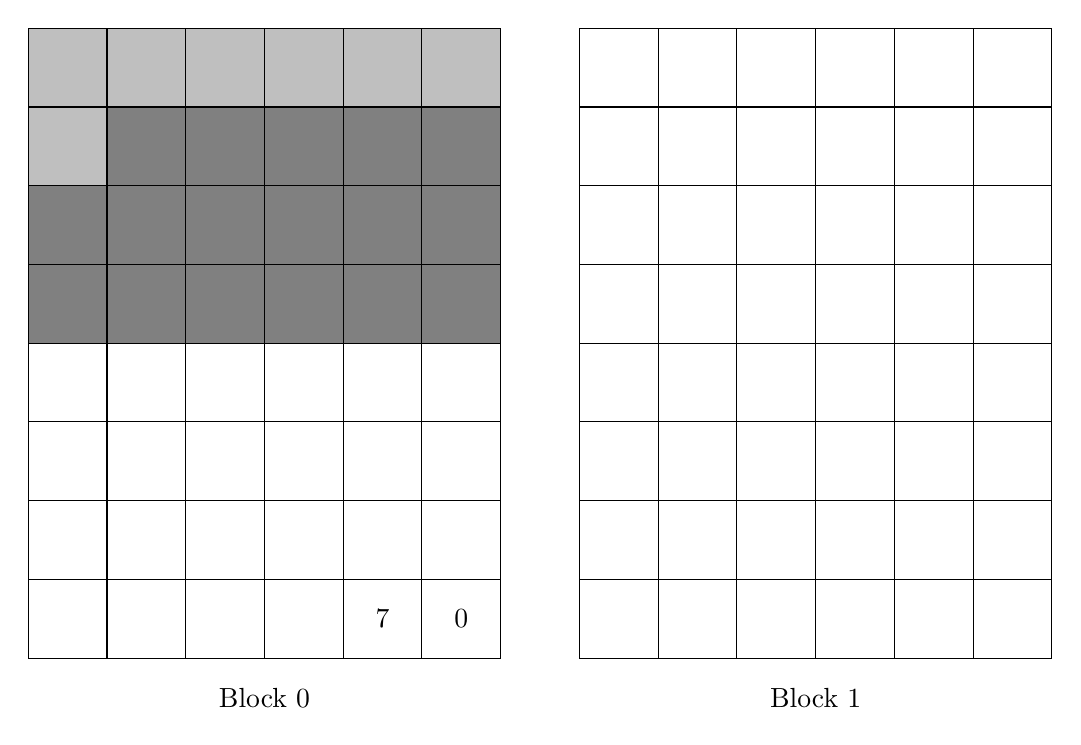
\begin{tikzpicture}
		% Sätze
		\fill[fill=lightgray] (0,8) rectangle +(6,-2);
		\fill[fill=gray] (1,7) rectangle +(5,-1) (0,6) rectangle +(6,-2);

		% Index
		\node at (4.5,0.5) {7};
		\node at (5.5,0.5) {0};

		% Gitter
		\draw (0,0) grid +(6,8) (7,0) grid +(6,8);
		\node at (3,-0.5) {Block~0};
		\node at (10,-0.5) {Block~1};
	\end{tikzpicture}
	\end{center}

	\begin{solution}
	\begin{center}
	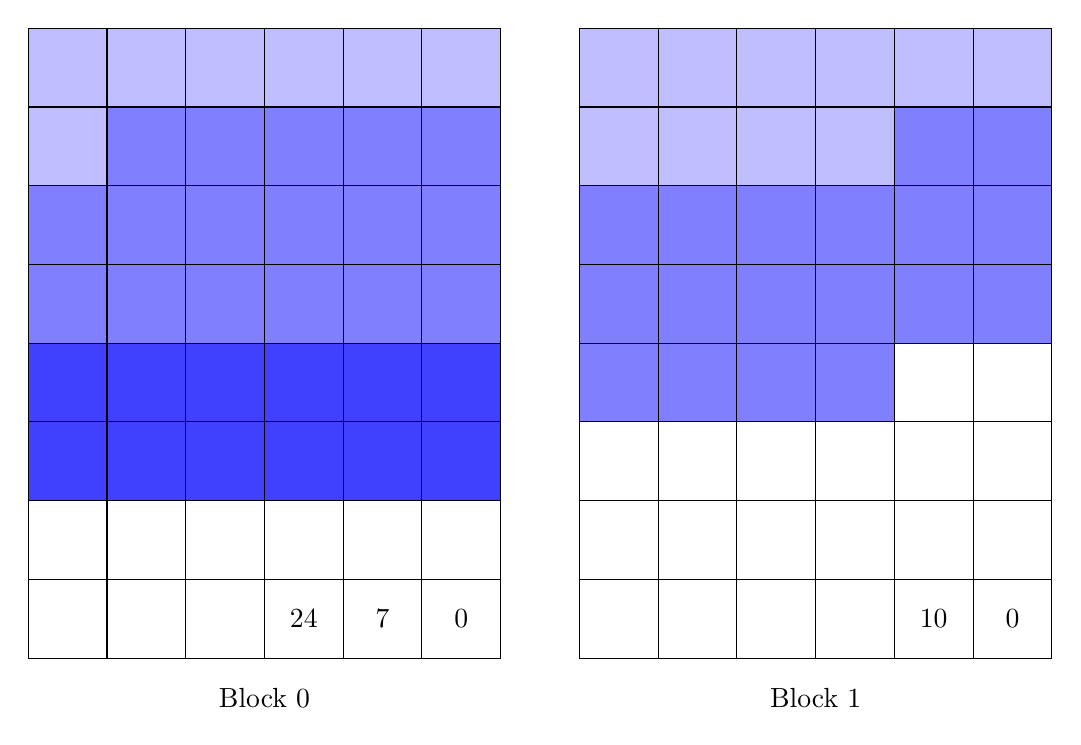
\begin{tikzpicture}
		% Sätze Block 0
		\fill[fill=blue!25] (0,8) rectangle +(6,-2);
		\fill[fill=blue!50] (1,7) rectangle +(5,-1) (0,6) rectangle +(6,-2);
		\fill[fill=blue!75] (0,4) rectangle +(6,-2);

		% Sätze Block 1
		\fill[fill=blue!25] (7,8) rectangle +(6,-1) (7, 7) rectangle +(4, -1);
		\fill[fill=blue!50] (11,7) rectangle +(2,-1) (7,6) rectangle +(6,-2) (7, 4) rectangle +(4, -1);

		% Index Block 0
		\node at (3.5,0.5) {24};
		\node at (4.5,0.5) {7};
		\node at (5.5,0.5) {0};

		% Index Block 1
		\node at (12.5,0.5) {0};
		\node at (11.5,0.5) {10};

		% Gitter
		\draw (0,0) grid +(6,8) (7,0) grid +(6,8);
		\node at (3,-0.5) {Block~0};
		\node at (10,-0.5) {Block~1};
	\end{tikzpicture}
	\end{center}
	12: TID(0, 2), 10: TID(1, 0), 18: TID(1, 1)
	\end{solution}

\begin{beamerText}
\pagebreak
\begin{itemize}
	\item Größe eines Indexeintrags 1~Byte
	\item Größe einer TID 2~Byte
	\end{itemize}
\end{beamerText}

	\item \label{TIDVerlaengerung} Betrachten Sie die folgende Skizze: Block~0 hat zusätzlich zur obigen Ausgangssituation den Satz TID(0, 2) mit der Länge 16 bekommen. Block~1 enthält Satz TID(1, 0) mit der Länge 8.

	Satz TID(0, 0) soll auf die Länge 12 und anschließend Satz TID(0, 1) auf die Länge 23 vergrößert  werden. Zeichnen Sie jeweils die nach den Verlängerungen entstehenden Situationen und geben Sie wieder die zugehörigen TIDs an.

	\begin{center}
	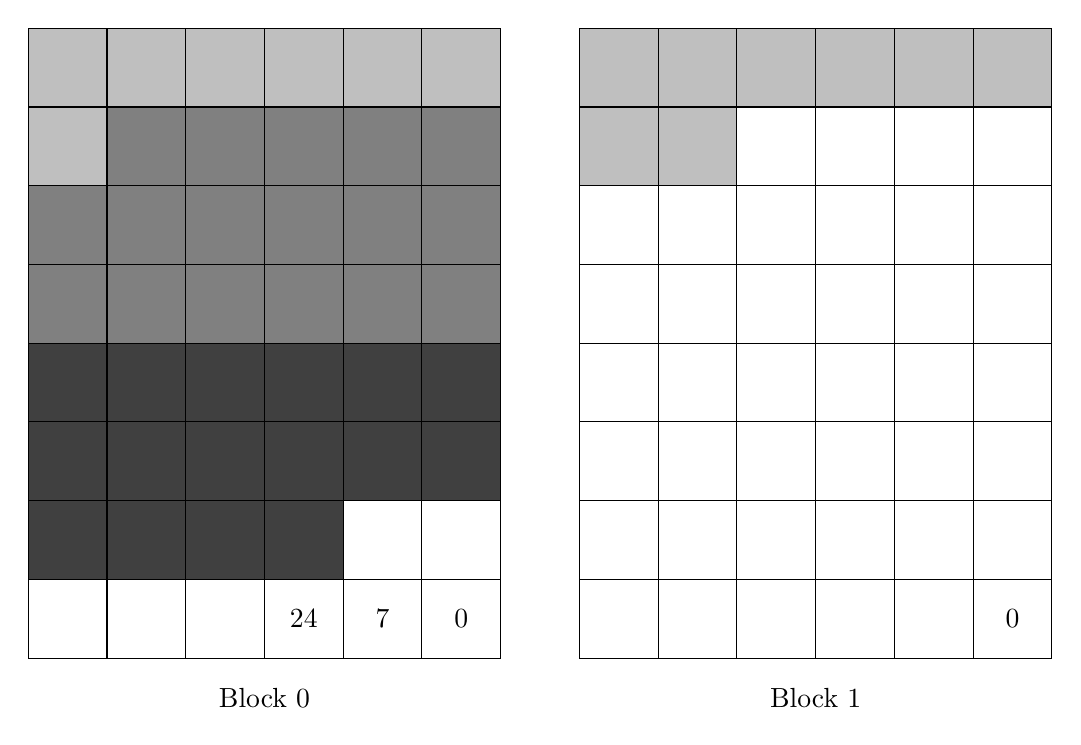
\begin{tikzpicture}
		% Sätze Block 0
		\fill[fill=lightgray] (0,8) rectangle +(6,-2);
		\fill[fill=gray] (1,7) rectangle +(5,-1) (0,6) rectangle +(6,-2);
		\fill[fill=darkgray] (0,4) rectangle +(6,-2) (0,2) rectangle +(4,-1);

		% Sätze Block 1
		\fill[fill=lightgray] (7,8) rectangle +(6,-1) (7,7) rectangle +(2,-1);

		% Index Block 0
		\node at (3.5,0.5) {24};
		\node at (4.5,0.5) {7};
		\node at (5.5,0.5) {0};

		% Index Block 1
		\node at (12.5,0.5) {0};

		% Gitter
		\draw (0,0) grid +(6,8) (7,0) grid +(6,8);
		\node at (3,-0.5) {Block~0};
		\node at (10,-0.5) {Block~1};
	\end{tikzpicture}
	\end{center}

	\begin{solution}
	Verlängerung von TID(0, 0) auf 12: Block 0 ist komplett gefüllt.
	\begin{center}
	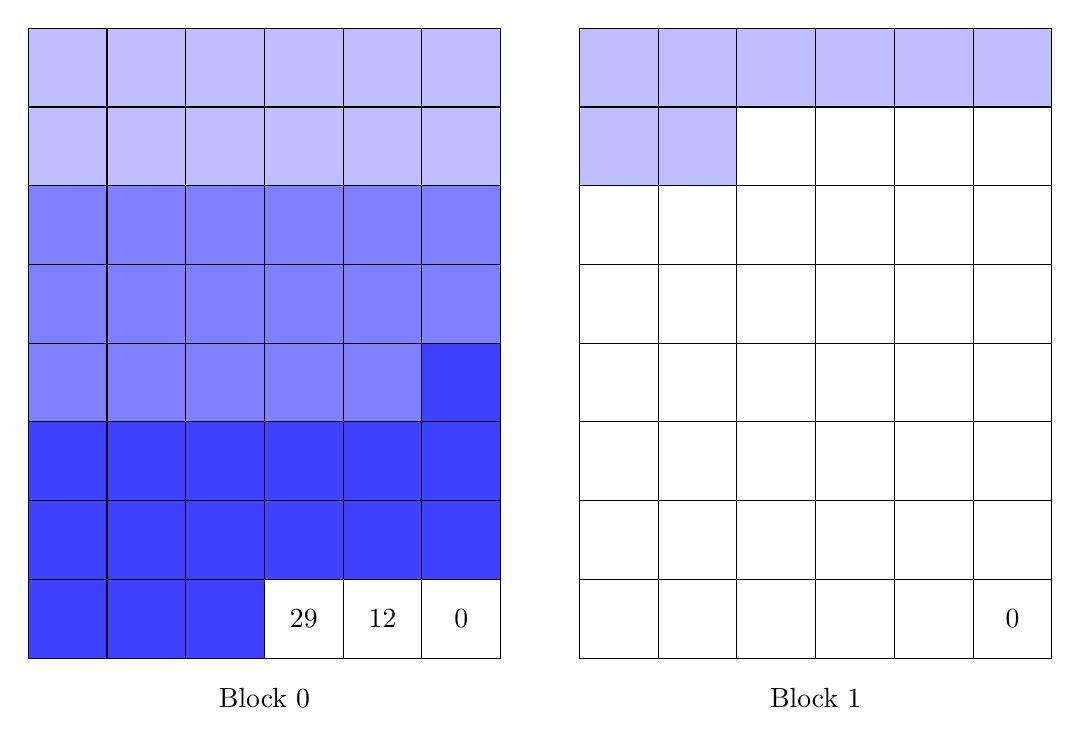
\begin{tikzpicture}
		% Sätze Block 0
		\fill[fill=blue!25] (0,8) rectangle +(6,-2);
		\fill[fill=blue!50] (0,6) rectangle +(6,-3);
		\fill[fill=blue!75] (5,4) rectangle +(1,-1) (0, 3) rectangle +(6, -2) (0, 1) rectangle (3, 0);

		% Sätze Block 1
		\fill[fill=blue!25] (7,8) rectangle +(6,-1) (7, 7) rectangle +(2, -1);

		% Index Block 0
		\node at (3.5,0.5) {29};
		\node at (4.5,0.5) {12};
		\node at (5.5,0.5) {0};

		% Index Block 1
		\node at (12.5,0.5) {0};

		% Gitter
		\draw (0,0) grid +(6,8) (7,0) grid +(6,8);
		\node at (3,-0.5) {Block~0};
		\node at (10,-0.5) {Block~1};
	\end{tikzpicture}
	\end{center}

	7 $\rightarrow$ 12: TID(0, 0), 17: TID(0, 1), 16: TID(0, 2)

	Verlängerung von TID(0, 1) auf 23: Freispeicherverwaltung signalisiert, dass Block~0 komplett gefüllt ist $\Rightarrow$ Überlaufsatz
	\begin{center}
	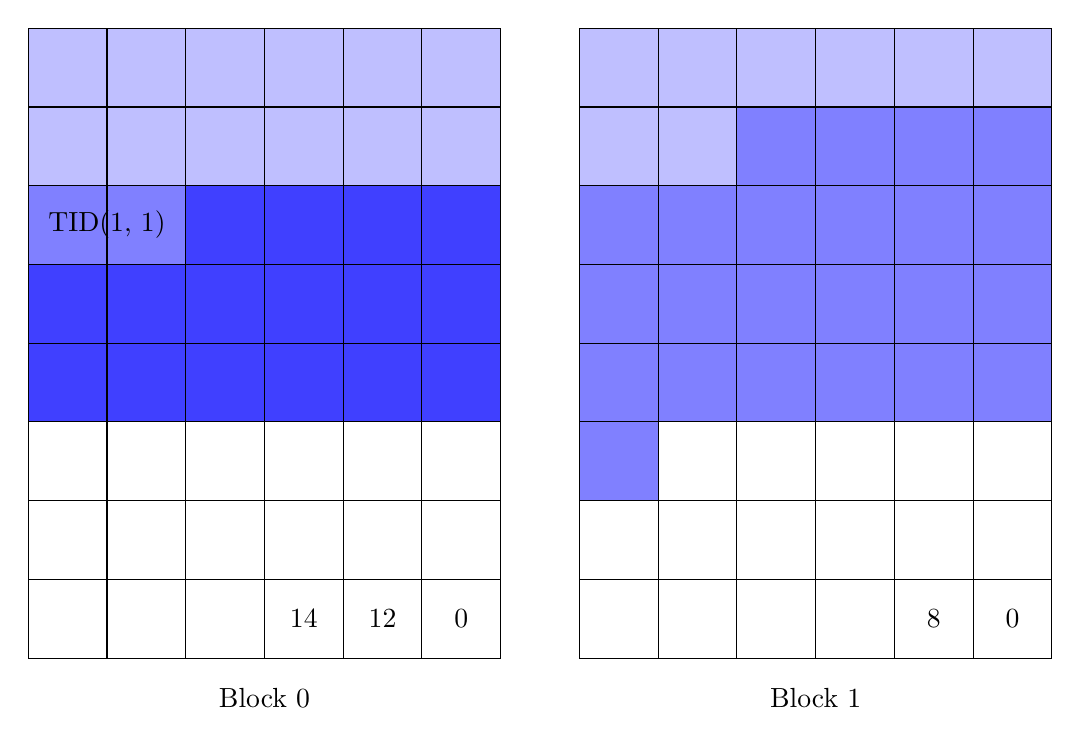
\begin{tikzpicture}
		% Sätze Block 0
		\fill[fill=blue!25] (0,8) rectangle +(6,-2);
		\fill[fill=blue!50] (0,6) rectangle +(2,-1);
		\fill[fill=blue!75] (2,6) rectangle +(4,-1) (0, 5) rectangle +(6, -2);

		% Sätze Block 1
		\fill[fill=blue!25] (7,8) rectangle +(6,-1) (7, 7) rectangle +(2, -1);
		\fill[fill=blue!50] (9,7) rectangle +(4,-1) (7, 6) rectangle +(6, -3) (7, 3) rectangle +(1, -1);

		% Index Block 0
		\node at (3.5,0.5) {14};
		\node at (4.5,0.5) {12};
		\node at (5.5,0.5) {0};

		% Index Block 1
		\node at (1,5.5) {TID(1, 1)};
		\node at (11.5,0.5) {8};
		\node at (12.5,0.5) {0};

		% Gitter
		\draw (0,0) grid +(6,8) (7,0) grid +(6,8);
		\node at (3,-0.5) {Block~0};
		\node at (10,-0.5) {Block~1};
	\end{tikzpicture}
	\end{center}

	12: TID(0, 0), 17 $\rightarrow$ 23: TID(0, 1), 16: TID(0, 2)

	Hinweis: Es ist vermutlich implementierungsabhängig, ob Block~0 gleich reorganisiert wird, d.h. ob TID(0, 2) nach vorne geschoben wird.
	\end{solution}
\begin{beamerText}
\pagebreak
\begin{itemize}
	\item Größe eines Indexeintrags 1~Byte
	\item Größe einer TID 2~Byte
	\end{itemize}
\end{beamerText}

	\item \label{TID_Fragment} Nach den beiden Satzvergrößerungen aus Teilaufgabe \ref{TIDVerlaengerung}) soll noch ein Satz der Länge 57 eingefügt werden. Zeichnen Sie die entstehende Situation und geben Sie die zugehörige TID des Satzes an. Gehen Sie davon aus, dass in Block~2 noch keine Sätze abgelegt sind.

\begin{normalText}
	Wenn ein einzufügender Satz die maximale Blockgröße überschreitet, muss er fragmentiert werden. Fragmente sind normalerweise so groß wie der maximal nutzbare Speicher eines Blocks, nur das letzte Fragment eines Satzes darf kleiner sein. Das bedeutet, die Fragmente eines Satzes haben alle die maximal nutzbare Speichergröße und werden jeweils in neue, unbefüllte Blöcke abgelegt, nur das letzte Fragment kann, falls es einen bereits teilweise gefüllten Block mit ausreichend freiem Speicher gibt, in diesem abgelegt werden. Der Zugriff auf einen solchen Satz erfolgt transparent, d.\,h. die Fragmente sind nach außen hin nicht sichtbar.

	Legen Sie in dieser Teilaufgabe zusätzlich zu den bisher in den Blöcken abgelegten Informationen einen Fragmentierungs-Header der Größe 2~Byte vor den Fragmenten eines Satzes mit ab. Dieser zeigt auf das nächste Fragment des Satzes. Wird auch vor dem letzten Fragment ein Fragmentierungs-Header benötigt?
\end{normalText}

	\begin{center}
	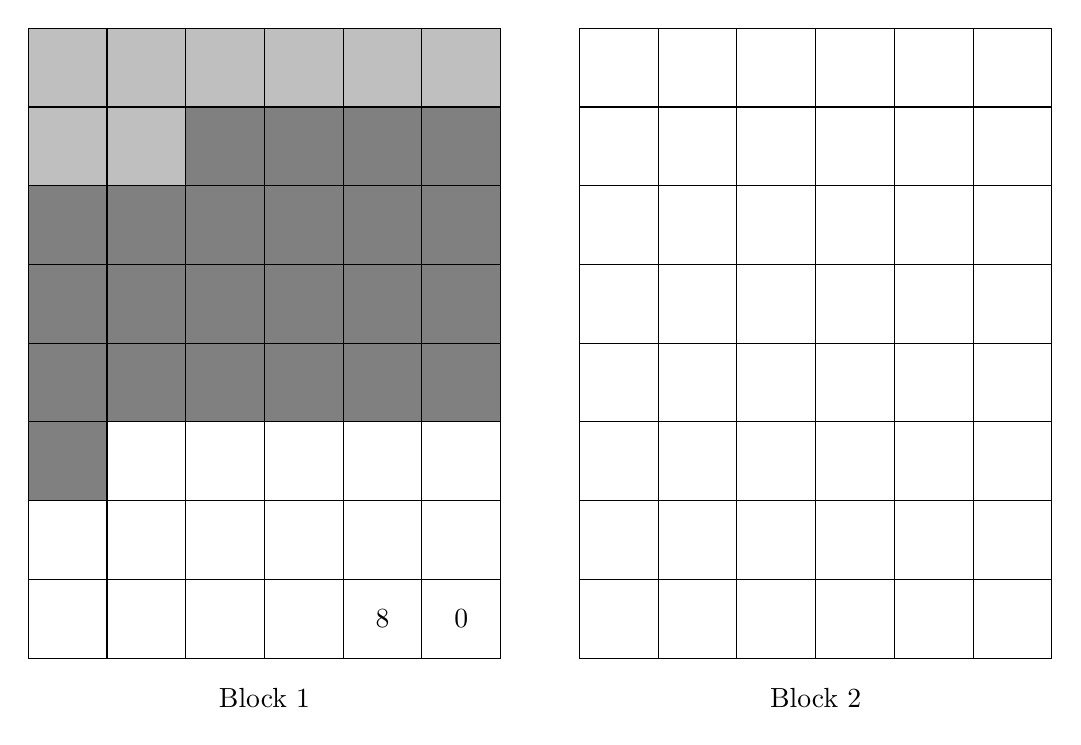
\begin{tikzpicture}
		% Sätze Block 1
		\fill[fill=lightgray] (0,8) rectangle +(6,-2);
		\fill[fill=gray] (2,7) rectangle +(4,-1) (0,6) rectangle +(6,-3) (0,3) rectangle +(1,-1);

		% Index Block 1
		\node at (5.5,0.5) {0};
		\node at (4.5,0.5) {8};
		% Gitter
		\draw (0,0) grid +(6,8) (7,0) grid +(6,8);
		\node at (3,-0.5) {Block~1};
		\node at (10,-0.5) {Block~2};
	\end{tikzpicture}
	\end{center}

\begin{beamerText}
	\pagebreak
	Wenn ein einzufügender Satz die maximale Blockgröße überschreitet, muss er fragmentiert werden. Fragmente sind normalerweise so groß wie der maximal nutzbare Speicher eines Blocks, nur das letzte Fragment eines Satzes darf kleiner sein. Das bedeutet, die Fragmente eines Satzes haben alle die maximal nutzbare Speichergröße und werden jeweils in neue, unbefüllte Blöcke abgelegt, nur das letzte Fragment kann, falls es einen bereits teilweise gefüllten Block mit ausreichend freiem Speicher gibt, in diesem abgelegt werden. Der Zugriff auf einen solchen Satz erfolgt transparent, d.\,h. die Fragmente sind nach außen hin nicht sichtbar.

	Legen Sie in dieser Teilaufgabe zusätzlich zu den bisher in den Blöcken abgelegten Informationen einen Fragmentierungs-Header der Größe 2~Byte vor den Fragmenten eines Satzes mit ab. Dieser zeigt auf das nächste Fragment des Satzes. Wird auch vor dem letzten Fragment ein Fragmentierungs-Header benötigt?
\end{beamerText}

	\begin{solution}
	Das letzte Fragment benötigt keinen Fragmentierungs-Header, da ja kein weiteres Fragment mehr kommt.

	Fragmentiere Satz der Länge 57 in 2 Fragmente der Größe 45 (= Blockgröße – 1~Byte Indexeintrag – 2~Byte Fragmentierungs-Header) und 12 (= Rest). Lege Fragment der Größe 45 in neuen Block 2. Fragment der Größe 12 passt noch in Block 1.
	\begin{center}
	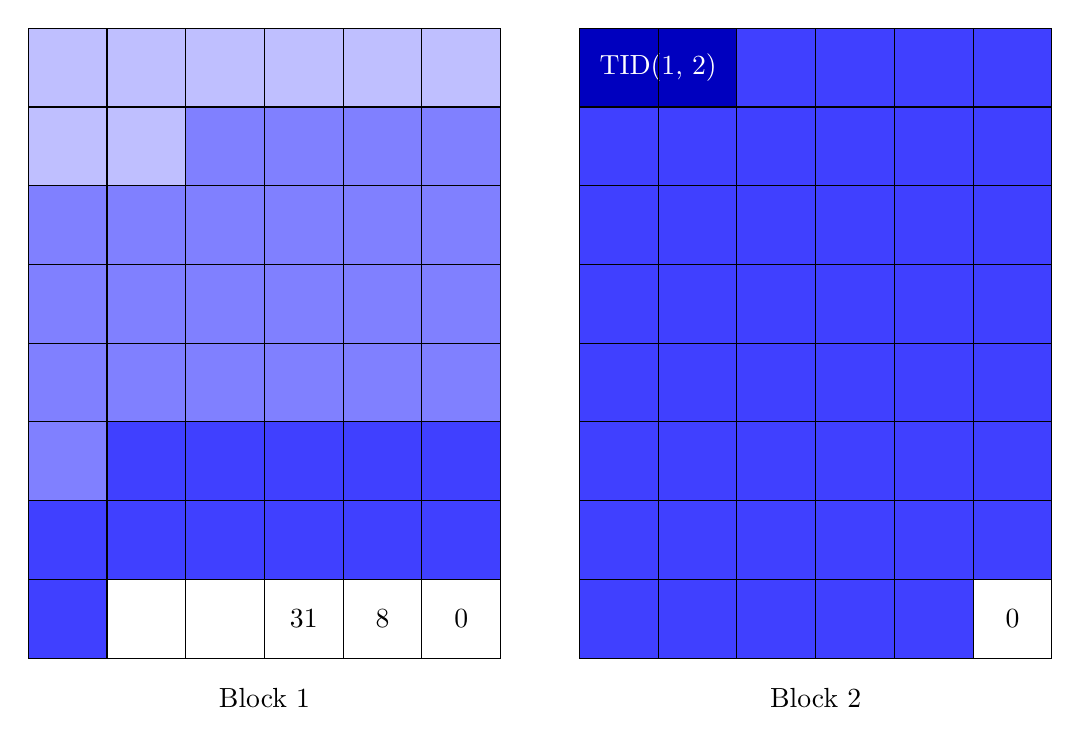
\begin{tikzpicture}
		% Sätze Block 1
		\fill[fill=blue!25] (0,8) rectangle +(6,-2);
		\fill[fill=blue!50] (2,7) rectangle +(4,-1) (0,6) rectangle +(6,-3) (0,3) rectangle +(1,-1);
		\fill[fill=blue!75] (1, 3) rectangle +(5, -1) (0, 2) rectangle +(6, -1) (0, 1) rectangle +(1, -1);
		% Index Block 1
		\node at (5.5,0.5) {0};
		\node at (4.5,0.5) {8};
		\node at (3.5, 0.5) {31};

		%Sätze Block 2
		\fill[fill=blue!75!black] (7, 8) rectangle +(2, -1);
		\fill[fill=blue!75] (9,8) rectangle +(4, -1) (7, 7) rectangle +(6, -6) (7, 1) rectangle +(5, -1);

		%Index Block 2
		\node at (12.5, 0.5) {0};
		\node at (8,7.5) {\color{white}TID(1, 2)};

		% Gitter
		\draw (0,0) grid +(6,8) (7,0) grid +(6,8);
		\node at (3,-0.5) {Block~1};
		\node at (10,-0.5) {Block~2};
	\end{tikzpicture}
	\end{center}

	57: TID(2, 0)

	Wichtig ist die Erkenntnis, dass der Zeiger von einem Fragment auf das nächste oder von der ursprünglichen Satzposition auf die tatsächliche wieder eine TID ist.
	\end{solution}

	\item \label{TID_erw_red} Betrachten \selbst Sie die aus Teilaufgabe \ref{TID_Fragment}) resultierende Situation.
	Erweitern Sie nun den Satz mit TID(0,1) auf die Länge 26.
	Verkleinern Sie anschließend den Satz mit TID(2,0) auf die Länge 10.

	\begin{note}
		Für die Umstrukturierung des Satzes mit TID(0,1) benötigen wir zunächst die Blöcke 0 und 1.

		Ausgangssituation

		\begin{center}
			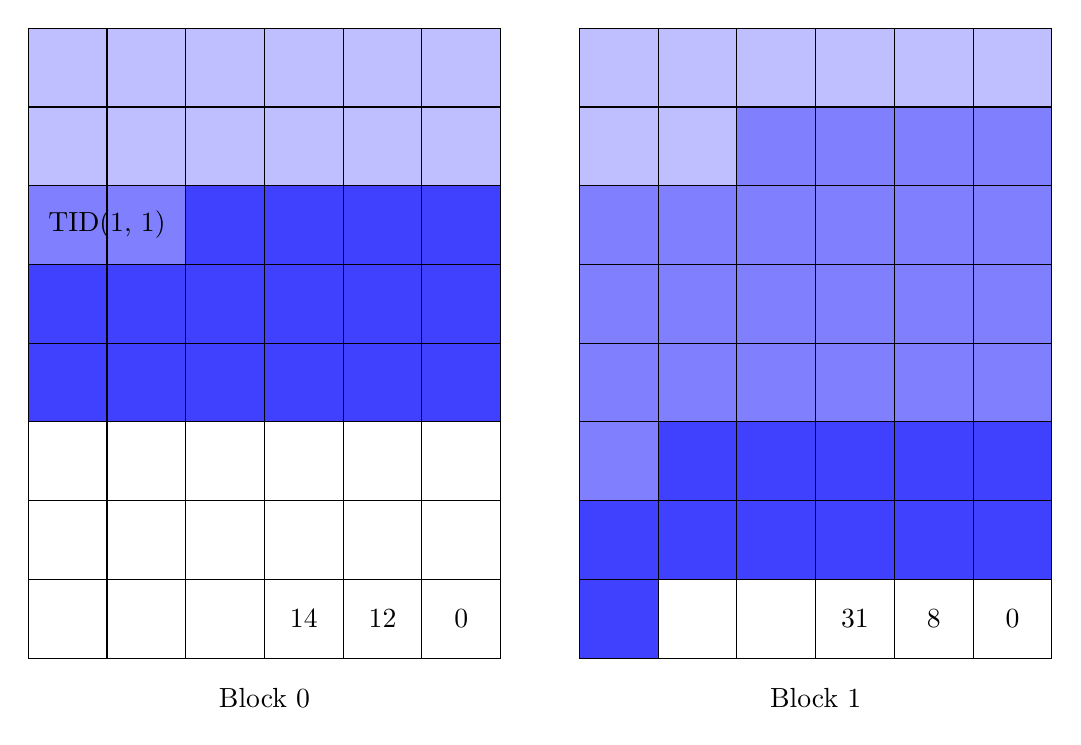
\begin{tikzpicture}
				% Sätze Block 0
				\fill[fill=blue!25] (0,8) rectangle +(6,-2);
				\fill[fill=blue!50] (0,6) rectangle +(2,-1);
				\fill[fill=blue!75] (2,6) rectangle +(4,-1) (0, 5) rectangle +(6, -2);

				% Sätze Block 1


				\fill[fill=blue!25] (7,8) rectangle +(6,-2);
				\fill[fill=blue!50] (9,7) rectangle +(4,-1) (7,6) rectangle +(6,-3) (7,3) rectangle +(1,-1);
				\fill[fill=blue!75] (8, 3) rectangle +(5, -1) (7, 2) rectangle +(6, -1) (7, 1) rectangle +(1, -1);
				% Index Block 0
				\node at (3.5,0.5) {14};
				\node at (4.5,0.5) {12};
				\node at (5.5,0.5) {0};

				% Index Block 1
				\node at (1,5.5) {TID(1, 1)};
				\node at (10.5,0.5) {31};
				\node at (11.5,0.5) {8};
				\node at (12.5,0.5) {0};
				% Gitter
				\draw (0,0) grid +(6,8) (7,0) grid +(6,8);
				\node at (3,-0.5) {Block~0};
				\node at (10,-0.5) {Block~1};
			\end{tikzpicture}
		\end{center}
		Bei der Verlängerung von TID(0,1) signalisiert die Freispeicherverwaltung, dass Block 1 zu klein ist $\Rightarrow$ Überlaufsatz.

		Hinweis: Es ist vermutlich implementierungsabhängig, ob Block~1 gleich reorganisiert wird, d.h. ob TID(1, 2) nach vorne geschoben wird.

		Situation nach dem Verlängern:

		\begin{center}
			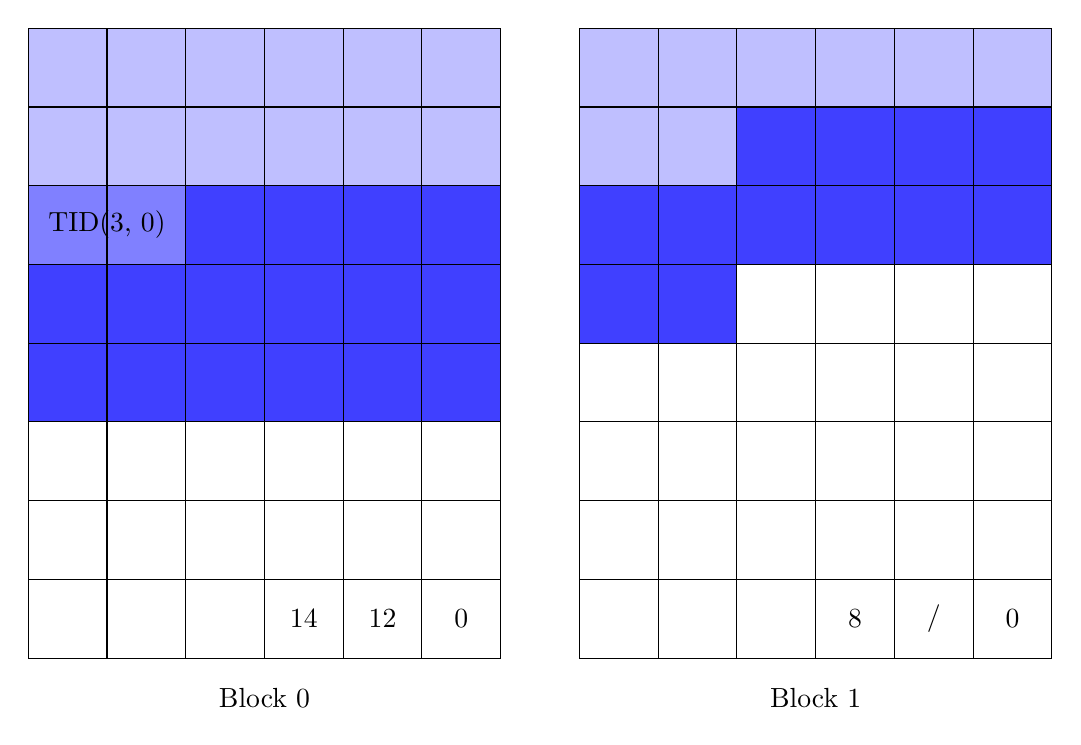
\begin{tikzpicture}
			% Sätze Block 0
			\fill[fill=blue!25] (0,8) rectangle +(6,-2);
			\fill[fill=blue!50] (0,6) rectangle +(2,-1);
			\fill[fill=blue!75] (2,6) rectangle +(4,-1) (0, 5) rectangle +(6, -2);

			% Sätze Block 1

			\fill[fill=blue!25] (7,8) rectangle +(6,-2);

			\fill[fill=blue!75] (9, 7) rectangle +(4, -1) (7, 6) rectangle +(6, -1) (7, 5) rectangle +(2, -1);
			% Index Block 0
			\node at (3.5,0.5) {14};
			\node at (4.5,0.5) {12};
			\node at (5.5,0.5) {0};

			% Index Block 1
			\node at (1,5.5) {TID(3, 0)};
			\node at (10.5,0.5) {8};
			\node at (11.5,0.5) {/};
			\node at (12.5,0.5) {0};
			% Gitter
			\draw (0,0) grid +(6,8) (7,0) grid +(6,8);
			\node at (3,-0.5) {Block~0};
			\node at (10,-0.5) {Block~1};
			\end{tikzpicture}
		\end{center}
		\begin{center}
			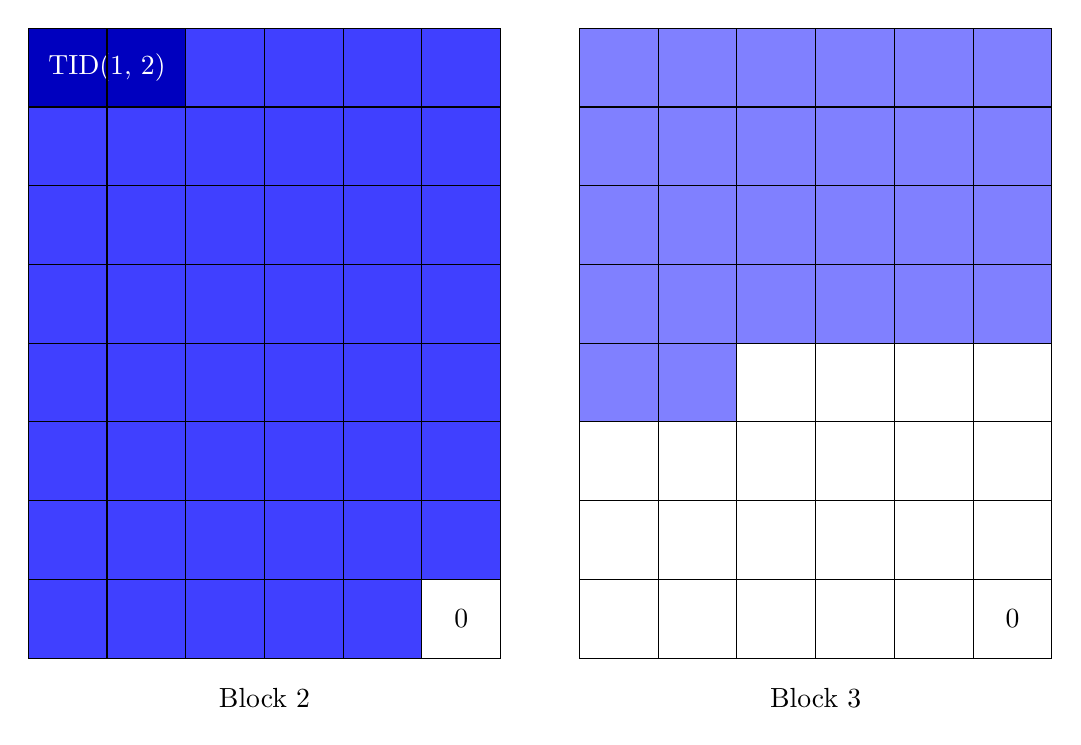
\begin{tikzpicture}
			%Sätze Block 2
			\fill[fill=blue!75!black] (0, 8) rectangle +(2, -1);
			\fill[fill=blue!75] (2,8) rectangle +(4, -1) (0, 7) rectangle +(6, -6) (0, 1) rectangle +(5, -1);

			%Sätze Block 3
			\fill[fill=blue!50] (7,8) rectangle +(6,-4) (7,4) rectangle +(2,-1);

			%Index Block 2
			\node at (5.5, 0.5) {0};
			\node at (1,7.5) {\color{white}TID(1, 2)};

			%Index Block 3
			\node at (12.5, 0.5) {0};
			% Gitter
			\draw (0,0) grid +(6,8) (7,0) grid +(6,8);
			\node at (3,-0.5) {Block~2};
			\node at (10,-0.5) {Block~3};

			\end{tikzpicture}
		\end{center}

		Wichtige ist hierbei, dass der Eintrag in TID(0,2) auf (3,0) umgebogen wird und TID(1,1) als ungültig markiert wird.

		Als Optimierung könnte zwischen ursprünglich nach außen sichtbaren gelöschten Sätzen und entfernten Überlaufsätzen unterschieden werden.
		Wenn deren Indexeinträge unterschiedlich als ungültig markiert werden, können TIDs von Überlaufsätzen, die nie nach außen gegeben wurden, wiederverwendet werden, was Indexeinträge spart.

		Für die Verkleinerung von TID(2,0) auf die Länge 10 verändern sich nun die Blöcke 1 und 2.

		Situation nach dem Verkleinern:

		\begin{center}
			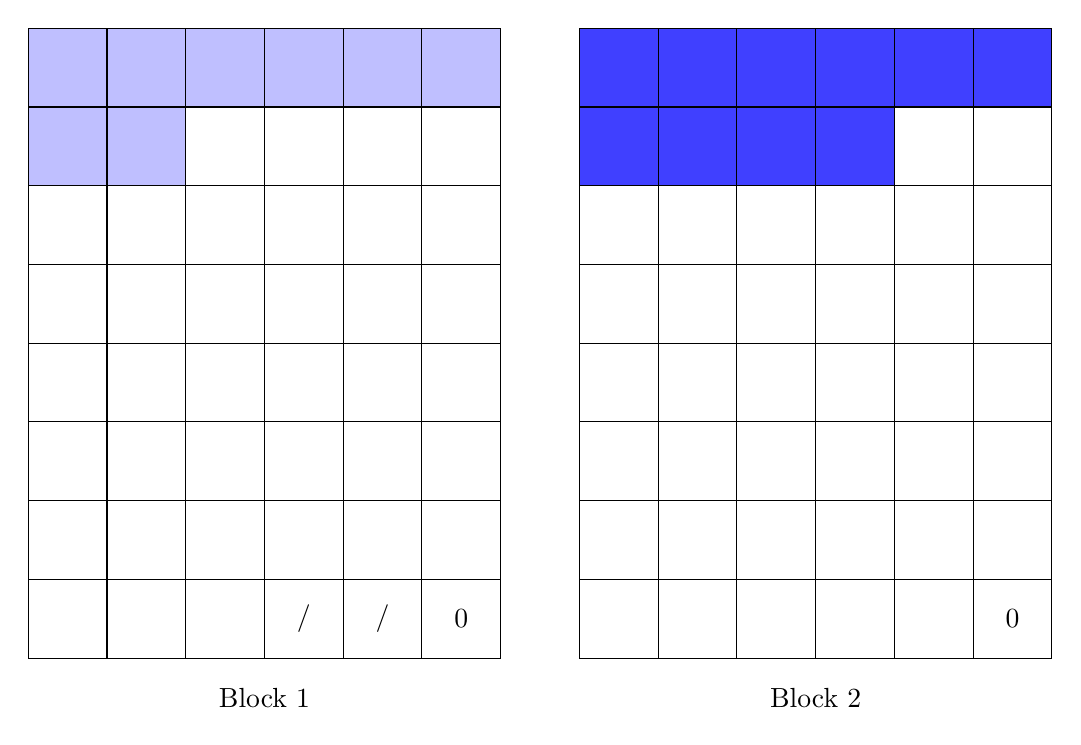
\begin{tikzpicture}
			% Sätze Block 1
			\fill[fill=blue!25] (0,8) rectangle +(6,-1) (0,7) rectangle +(2,-1);

			% Index Block 1
			\node at (5.5,0.5) {0};
			\node at (4.5,0.5) {/};
			\node at (3.5,0.5) {/};


			%Sätze Block 2

			\fill[fill=blue!75] (7,8) rectangle +(6, -1) (7, 7) rectangle +(4, -1);

			%Index Block 2
			\node at (12.5, 0.5) {0};

			% Gitter
			\draw (0,0) grid +(6,8) (7,0) grid +(6,8);
			\node at (3,-0.5) {Block~1};
			\node at (10,-0.5) {Block~2};
			\end{tikzpicture}
		\end{center}
	\end{note}
\end{enumerate}



\beamertxt{\pagebreak}
\section{TID-Konzept}
\begin{enumerate}[a)]
	\item Wie erkennt man, ob es sich beim Blockinhalt um Nutzdaten, eine TID, einen Indexeintrag, einen Fragmentierungsheader oder einen gelöschten Eintrag handelt?

	\begin{solution}
	\begin{itemize}
		\item Indexeinträge beginnen -- im Vergleich mit den Nutzdaten -- am jeweils anderen Ende eines Blocks.
		In unseren Beispielen ist das immer das hintere Ende.
		Man muss beim Lesen mit den Indexeinträgen beginnen, also wissen, an welchem Ende sie sich befinden.
		Und man muss wissen, wie viele Indexeinträge es überhaupt gibt.
		Dazu könnte man z.\,B.\ die Anzahl der Indexeinträge zu Beginn des Indexes ablegen.

		\item Ob ein von einem Index referenzierter Satz Nutzdaten, einen Verweis oder ein Satzfragment enthält, muss irgendwo gespeichert werden.
		Eine Möglichkeit ist, jedem Satz einen Header voranzustellen und diese Information darin zu speichern.
		Ein anderer Ansatz ist, z.\,B.\ bei Indexeinträgen der Größe 2\,Byte die Blockgröße auf 8\,KiB zu beschränken.
		Dadurch bleibt noch drei Bit in jedem Indexeintrag übrig.
		In den ersten beiden kann gespeichert werden, ob der Satz einen Verweis bzw. Nutzdaten enthält oder nicht.
		Hierdurch ergeben sich nun mehrere Kombinationen:
		\begin{description}
			\item[00] Satz gelöscht
			\item[01] Satz enthält nur Nutzdaten
			\item[10] Satz enthält nur einen Verweis
			\item[11] Satz enthält einen Verweis und Nutzdaten, also ein Satzfragment mit Fragmentierungsheader
		\end{description}
		Lediglich das letzte Fragment eines fragmentierten Satzes wird mit dieser Methode nicht eindeutig als solches erkannt sondern kann mit normalen Nutzdaten verwechselt werden.
		Hierfür eignet sich dann das letzte freie Bit.
	\end{itemize}
	\end{solution}

	\begin{note}
	Natürlich sind jeweils auch andere Lösungen und verschiedene Optimierungen denkbar.
	\end{note}


	\item Unter welchen Bedingungen kann man beim TID-Konzept Blöcke durch das verschieben von Sätzen einsparen? Wie kann man dabei vorgehen?
	\label{TID_Zusammenfassen}

	\begin{solution}
	Verkleinern ist bei TID fast unmöglich, vor allem, wenn man (wie Oracle) die TIDs an den Benutzer herausgibt.

	Wenn noch ein Satz existiert, der zunächst in einem hinteren Block stand, so muss in diesem Block der Zeiger auf die tatsächliche Adresse beibehalten werden und der Block wird noch benötigt.
	Verschiebt man den Satz und ändert die TID, muss man das in allen Strukturen nachziehen, die auf diese TID verweisen (v.\,a. Indizes).
	Das ist zwar prinzipiell möglich, aber mit enormem Aufwand verbunden.
	\end{solution}

  \item In \deepen wie weit kann man die resultierende Dateigröße von Aufgabe \ref{sec:TID_angewandt1}\,\ref{TID_erw_red}) optimieren?

	\begin{note}
		Den Satz mit TID(3,0) kann man in den Block 1 kopieren, wenn man die TID(0,1) entsprechend anpasst.

		Das Verschieben des Satzes mit TID(2,0) würde keine Blockersparnis bringen, da Block 2 für die Stabilität der TID Einträge erhalten bleiben muss.
	\end{note}


	\item Eine alternative Möglichkeit zur Satzorganisation ist die sogenannte Database Key Translation Table (DBTT).
	Hierbei wird ein k Blöcke großes Feld verwaltet, das zu jeder Satznummer die Blocknummer und die Byte-Positionen enthält.

	Beim Einfügen wird stets eine neue Satznummer vergeben, beim Löschen die entsprechende Satznummer als ungültig markiert.
	Es handelt sich um ein stabiles Verfahren, d.\,h. Satznummern bleiben bei Verschiebungen unverändert, da lediglich der Eintrag des Satzes im Feld verändert werden muss.
	Dieser Database Key ist eine \emph{nicht sprechende Adresse}.	Das Feld kann am Anfang oder am Ende der Datei oder als separate Datei gespeichert werden.

	Was sind die Nachteile dieses Konzepts, und wie löst das TID-Konzept diese?

	\begin{solution}
	Nachteile:
	\begin{itemize}
		\item Ein Zugriff erfordert immer mindestens zwei Blockzugriffe: einen für das Feld, einen für die Nutzdaten.
		Bei TID kommt man (ohne Überlauf) mit einem Blockzugriff aus.
		\item Will man einen Satz in einem Block oder auch über Blockgrenzen hinweg verschieben, so muss man auch das Feld ändern.
		Das kann bei häufigen Änderungen oder hoher Nebenläufigkeit zu Engpässen führen, da das Feld ja persistent auf das Laufwerk geschrieben werden muss.
		Bei TID muss nur in den betroffenen Blöcken (Ursprungsblock und ggf. Überlaufblock) geschrieben werden
	\end{itemize}
	\end{solution}

	\begin{note}
	  Einen Vorteil hat das DBTT-Konzept aber auch: Blöcke lassen sich zusammenfassen (vgl. Aufgabe \ref{sec:TID_angewandt1}\,\ref{TID_Zusammenfassen}), da sich der Database Key durch das Verschieben eines Satzes in einen anderen Block nicht ändert.
	\end{note}
\end{enumerate}


\begin{selbstTest}
\section{TID angewandt 2}
Gehen Sie vom gleichen TID-Konzept wie in Aufgabe \ref{sec:TID_angewandt1} aus.
Die ersten vier Teilaufgaben bauen aufeinander auf.
\sol{Sie können deren Lösung in die leeren Blöcke auf Seite \pageref{fig:TID2_Blocks} eintragen.}

Zu Beginn befindet sich die Datei in folgendem Zustand:

\begin{center}
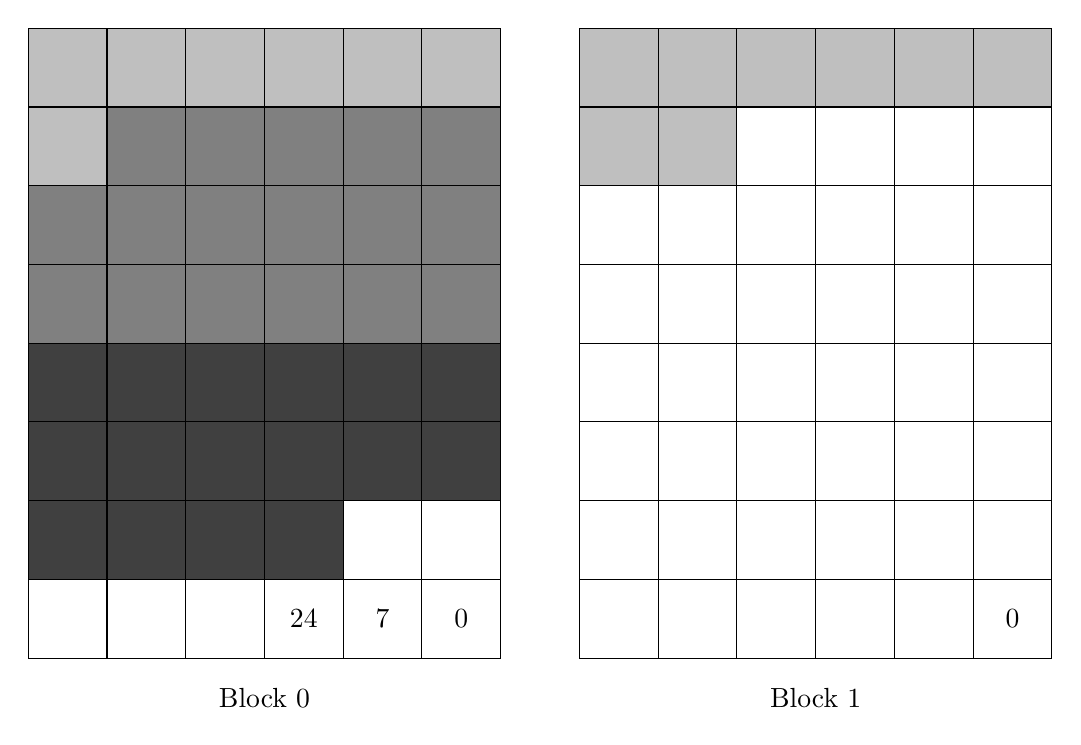
\begin{tikzpicture}
	% Sätze Block 0
	\fill[fill=lightgray] (0,8) rectangle +(6,-2);
	\fill[fill=gray] (1,7) rectangle +(5,-1) (0,6) rectangle +(6,-2);
	\fill[fill=darkgray] (0,4) rectangle +(6,-2) (0,2) rectangle +(4,-1);

	% Sätze Block 1
	\fill[fill=lightgray] (7,8) rectangle +(6,-1) (7,7) rectangle +(2,-1);

	% Index Block 0
	\node at (3.5,0.5) {24};
	\node at (4.5,0.5) {7};
	\node at (5.5,0.5) {0};

	% Index Block 1
	\node at (12.5,0.5) {0};

	% Gitter
	\draw (0,0) grid +(6,8) (7,0) grid +(6,8);

	\node at (3,-0.5) {Block~0};
	\node at (10,-0.5) {Block~1};
\end{tikzpicture}
\end{center}

\begin{normalText}
\begin{enumerate}[a)]
	\item Fügen Sie einen Satz der Größe 12 ein und notieren Sie sich die zugehörige TID.

	\begin{note}
		TID(1,1)
	\end{note}

	\item Vergrößern Sie den Satz mit TID(0,2) auf die Länge 22.
	\item Fügen Sie einen Satz mit Länge 48 ein und notieren Sie sich die zugehörige TID.

	\begin{note}
		TID(2,0)
	\end{note}

	\item Fügen Sie 5 Sätze der Länge 2 ein und notieren Sie sich die zugehörigen TIDs. Was fällt Ihnen hierbei auf?

	\begin{note}
		TID(0,4), TID(0,5), TID(0,6), TID(0,7), TID(0,8)

		Kleine Sätze verbrauchen viel Speicher für die Organisation.
	\end{note}

\begin{solution}
\begin{figure}
\begin{tikzpicture}
	\begin{note}
		% Sätze Block 0
		\fill[fill=blue!25] (0,17) rectangle +(6,-2);
		\fill[fill=blue!40] (1,16) rectangle +(5,-1) (0,15) rectangle +(6,-2);
		%b)
		\fill[fill=blue!50] (0,13) rectangle +(2,-1);
		%c)
		\filldraw[fill=blue!75] (2,13) rectangle + (3,-1);
		%d)
		\filldraw[fill=blue!20] (5,13) rectangle + (1,-1); %1
		\filldraw[fill=blue!20] (0,12) rectangle + (1,-1);
		\filldraw[fill=blue!60] (1,12) rectangle + (2,-1); %2
		\filldraw[fill=blue!30] (3,12) rectangle + (2,-1); %3
		\filldraw[fill=blue!70] (5,12) rectangle + (1,-1); %4
		\filldraw[fill=blue!70] (0,11) rectangle + (1,-1);
		\filldraw[fill=blue!40] (1,11) rectangle + (2,-1); %5


		% Sätze Block 1
		\fill[fill=blue!75] (7,17) rectangle +(6,-1) (7,16) rectangle +(2,-1);
		%a)
		\fill[fill=blue!25] (9,16) rectangle + (4,-1) (7,15) rectangle +(6,-1) (7,14) rectangle +(2,-1);
		%b)
		\fill[fill=blue!50] (9,14) rectangle +(4,-1) (7,13) rectangle +(6,-3);

		% Sätze Block 2
		%c)
		\fill[fill=blue!75!black] (0, 8) rectangle +(2, -1);
		\fill[fill=blue!75] (2,8) rectangle +(4, -1) (0, 7) rectangle +(6, -6) (0, 1) rectangle +(5, -1);
		% Index Block 0
		\node at (3.5,9.5) {24};
		\node at (4.5,9.5) {7};
		\node at (5.5,9.5) {0};
		%b)
		\node at (1,12.5) {TID(1,2)};
		%c)
		\node at (2.5, 9.5) {26};
		%d)
		\node at (1.5,9.5) {29}; %1
		\node at (0.5,9.5) {31}; %2
		\node at (5.5,10.5) {33}; %3
		\node at (4.5,10.5) {35}; %4
		\node at (3.5,10.5) {37}; %5
		% Index Block 1
		\node at (12.5,9.5) {0};
		%a)
		\node at (11.5,9.5){8};
		%b)
		\node at (10.5,9.5){20};

		%Index Block 2
		\node at (5.5, 0.5) {0};
		\node at (1,7.5) {\color{white}TID(0, 3)};
	\end{note}

	% Gitter
	\draw (0,0) grid +(6,8) (7,0) grid +(6,8) ;
	\draw (0,9) grid +(6,8) (7,9) grid +(6,8);
	\node at (3,8.5) {Block~0};
	\node at (10,8.5) {Block~1};
	\node at (3,-0.5) {Block~2};
	\node at (10,-0.5) {Block~3};
\end{tikzpicture}
\label{fig:TID2_Blocks}
\end{figure}
\end{solution}
\pagebreak

	\item Löschen Sie nun aus der folgenden Skizze den Satz mit TID(0,1).
	\begin{center}
		\begin{tikzpicture}
		% Sätze Block 0 Vorher
		\fill[fill=lightgray] (0,8) rectangle +(6,-2);
		\fill[fill=gray] (1,7) rectangle +(5,-1) (0,6) rectangle +(6,-2);
		\fill[fill=darkgray] (0,4) rectangle +(6,-2) (0,2) rectangle +(4,-1);

		% Index Block 0 Vorher
		\node at (3.5,0.5) {24};
		\node at (4.5,0.5) {7};
		\node at (5.5,0.5) {0};
		\begin{note}
		% Sätze Block 0 Nachher
		\fill[fill=blue!25] (7,8)  rectangle +(6,-2);
		\fill[fill=blue!50] (8,7) rectangle +(5,-1) (7,6) rectangle +(6,-1) (7,5) rectangle +(5,-1) ;

		% Index Block 0 Nachher
		\node at (12.5,0.5) {0};
		\node at (11.5,0.5) {/};
		\node at (10.5,0.5) {7};
		\end{note}
		% Gitter
		\draw (0,0) grid +(6,8) (7,0) grid +(6,8);

		\node at (3,-0.5) {Block~0~Vorher};
		\node at (10,-0.5) {Block~0~Nachher};


		\end{tikzpicture}
	\end{center}

	\begin{note}
		Hinweis: Es ist vermutlich implementierungsabhängig, ob Block~0 gleich reorganisiert wird, d.h. ob TID(0, 2) nach vorne geschoben wird.
	\end{note}
\end{enumerate}
\end{normalText}

\end{selbstTest}

\begin{deeper}
\section{Programmieraufgabe 2: SeqRecordFile}

\subsection{Aufgabenstellung}
\begin{enumerate}
	\item Implementieren Sie eine Klasse, die die Schnittstelle \beamertxt{\linebreak}\texttt{idb.record.SeqRecordFile} implementiert.
		Beachten Sie die Dokumentation der Methoden in der Schnittstelle.
	\item Tragen Sie den Konstruktor Ihrer Klasse in \texttt{idb.construct.Util} in der Methode \texttt{generateSeqRecordFile()} ein.
		Die Funktion soll den DBBuffer und eine BlockFile nehmen und eine \textbf{neue} SeqRecordFile zurückgeben.
		Beachten Sie, dass die BlockFile zu diesem Zeitpunkt schon geöffnet ist.
	\item Tragen Sie den Konstruktor Ihrer Klasse in \texttt{idb.construct.Util} in der Methode \texttt{rebuildSeqRecordFile()} ein.
		Die Funktion soll den DBBuffer und eine BlockFile nehmen und eine \textbf{existierende} SeqRecordFile vom Laufwerk laden.
		Beachten Sie, dass die BlockFile zu diesem Zeitpunkt schon geöffnet ist.
	\item Sorgen Sie dafür, dass Sie alle Tests aus der Klasse \texttt{SeqTests} erfüllen.
	Sie können diese Testfälle mit \lstinline|ant Meilenstein2| ausführen.
	\item Die Abgabe auf GitLab erfolgt zeitgleich mit der Abgabe der Zusatzaufgaben des nächsten Übungsblattes auf StudOn. Markieren Sie hierfür ihre Abgabe mit dem Tag "`Aufgabe-2"'.
\end{enumerate}

\subsection{Hinweise}
\begin{itemize}
	\item Im Gegensatz zur Vorlesung ist unsere SeqRecordfile eine List von Tupeln, keine Menge. Das bedeutet, dass die Ordnung erhalten bleiben muss.
	\item Achten Sie darauf, dass Sätze größer als ein Block sein können.
	\item Achten Sie darauf, dass Sie für das Auslesen der fragmentierten Sätze die Länge bereits kennen müssen.
		Es empfiehlt sich, die Länge der Sätze vor den eigentlichen Daten abzuspeichern.
	\item Zum Zugriff auf die BlockFile soll der \texttt{DBBuffer} verwendet werden.
	\item Ein \texttt{DataObject} ist eine Klasse, die sich um die Serialisierung und Deserialisierung kümmert.
	\item Ein \texttt{DataObject::size} kann sich beim Aufruf von \texttt{DataObject::read} verändern.
	\item Beim Aufruf von \texttt{DBString::copy} muss nicht zwangsläufig ein DBString zurückkommen, sondern ein beliebiges \texttt{DataObject}.
			Achten Sie darauf, dass ein Cast nicht erfolgreich sein muss.
	\item Beim fragmentierten Lesen eines \texttt{DataObjects} muss eine Liste von Tripel übergeben werden.
		Achten Sie darauf, keine \textit{use-after-free} nach \texttt{DBBuffer::unfix} zu begehen. (Dies wird die Testfälle fehlschlagen lassen.)
	\item Testen Sie Ihre Implementierung, indem Sie den Inhalt der Klasse \texttt{idb.Main} durch Testcode für ihre SeqRecordFile ersetzen.
		Setzen Sie \texttt{Main} auf den orginalen Zustand zurück, sobald Sie sich von der Korrektheit überzeugt haben.
	\item Zur Implementierung der View bietet sich die Verwendung einer inneren Klasse an, um Zugriff auf den Zustand der SeqRecordFile zu haben.
	\item Um das Schreiben von Tupeln zu beschleunigen, lohnt es sich, im ersten Block Metadaten abzulegen, in welchem Block an welcher Stelle der freie Platz anfängt.
	\item SeqRecordFile bietet keine Operation zum Löschen an und ist deswegen für die langfristige Speicherung nicht nützlich, sondern nur für spezifische Aufgaben in der Datenbank gedacht.
\end{itemize}

\end{deeper}
\end{document}
